\documentclass[11pt]{article}
\usepackage[utf8]{inputenc}
\usepackage{geometry}
\usepackage{graphicx}
\usepackage{hyperref}
\usepackage{amsmath}
\usepackage{listings}
\usepackage{xcolor}
\usepackage{float}

% Set page margins
\geometry{a4paper, margin=1in}

% Set up code listing style
\lstset{
    basicstyle=\ttfamily,
    commentstyle=\color{gray},
    keywordstyle=\color{blue},
    stringstyle=\color{red},
    showstringspaces=false,
    captionpos=b
}

\title{Development of a Sudoku Solver: C1 Research Computing Coursework}
\author{Vishal Jain}
\date{\today}

\begin{document}

\maketitle

\tableofcontents

\newpage

\section{Introduction}

\begin{quote}
    "Sudoku is a denial of service attack on human
  intellect" - Ben Laurie
\end{quote}

This report details the development of a Sudoku solver inline with the requirements of the C1 Research Computing coursework. The programme takes as input an incomplete grid in the form of a text file with a 9x9 grid of numbers with zero representing unknown values and `|`,`+`,`-` separating cells and , i.e.:


\begin{verbatim}
    $ cat input.txt
    000|007|000
    000|009|504
    000|050|169
    ---+---+---
    080|000|305
    075|000|290
    406|000|080
    ---+---+---
    762|080|000
    103|900|000
    000|600|000
    \end{verbatim}

and outputs the completed grid in the same form.

\subsection{Background and motivation}

Sudoku, a logic-based combinatorial number-placement puzzle, presents a paradigmatic example of a constraint satisfaction problem (CSP), a class of problems fundamental to the field of computer science. The puzzle's structure, consisting of a 9x9 grid divided into subgrids, adheres to stringent placement rules, thereby embodying the essence of CSPs where the objective is to find a solution that satisfies all given constraints.

This project, centered on the development of a Sudoku solver, is primarily motivated by the pedagogical value inherent in addressing such a well-defined and constrained problem space. Sudoku solvers exemplify the application of algorithmic strategies to a finite, yet non-trivial problem domain. This aligns with the core objectives of the C1 Research Computing coursework, which emphasizes the development of computational solutions that are both efficient and effective.

\section{Problem Decomposition}
To architect the Sudoku solver program, an initial flowchart was constructed to map out the high-level logical sequence. Each step of the flowchart was assigned a color based on its independence; steps that could be altered without impacting preceding steps received a unique color, whereas related, interdependent steps shared the same color. This method helped identify distinct, modular components within the program's workflow. The resulting color-coded flowchart is presented in Figure \ref{fig:solver_flowchart}.
\begin{figure}[H]
\centering
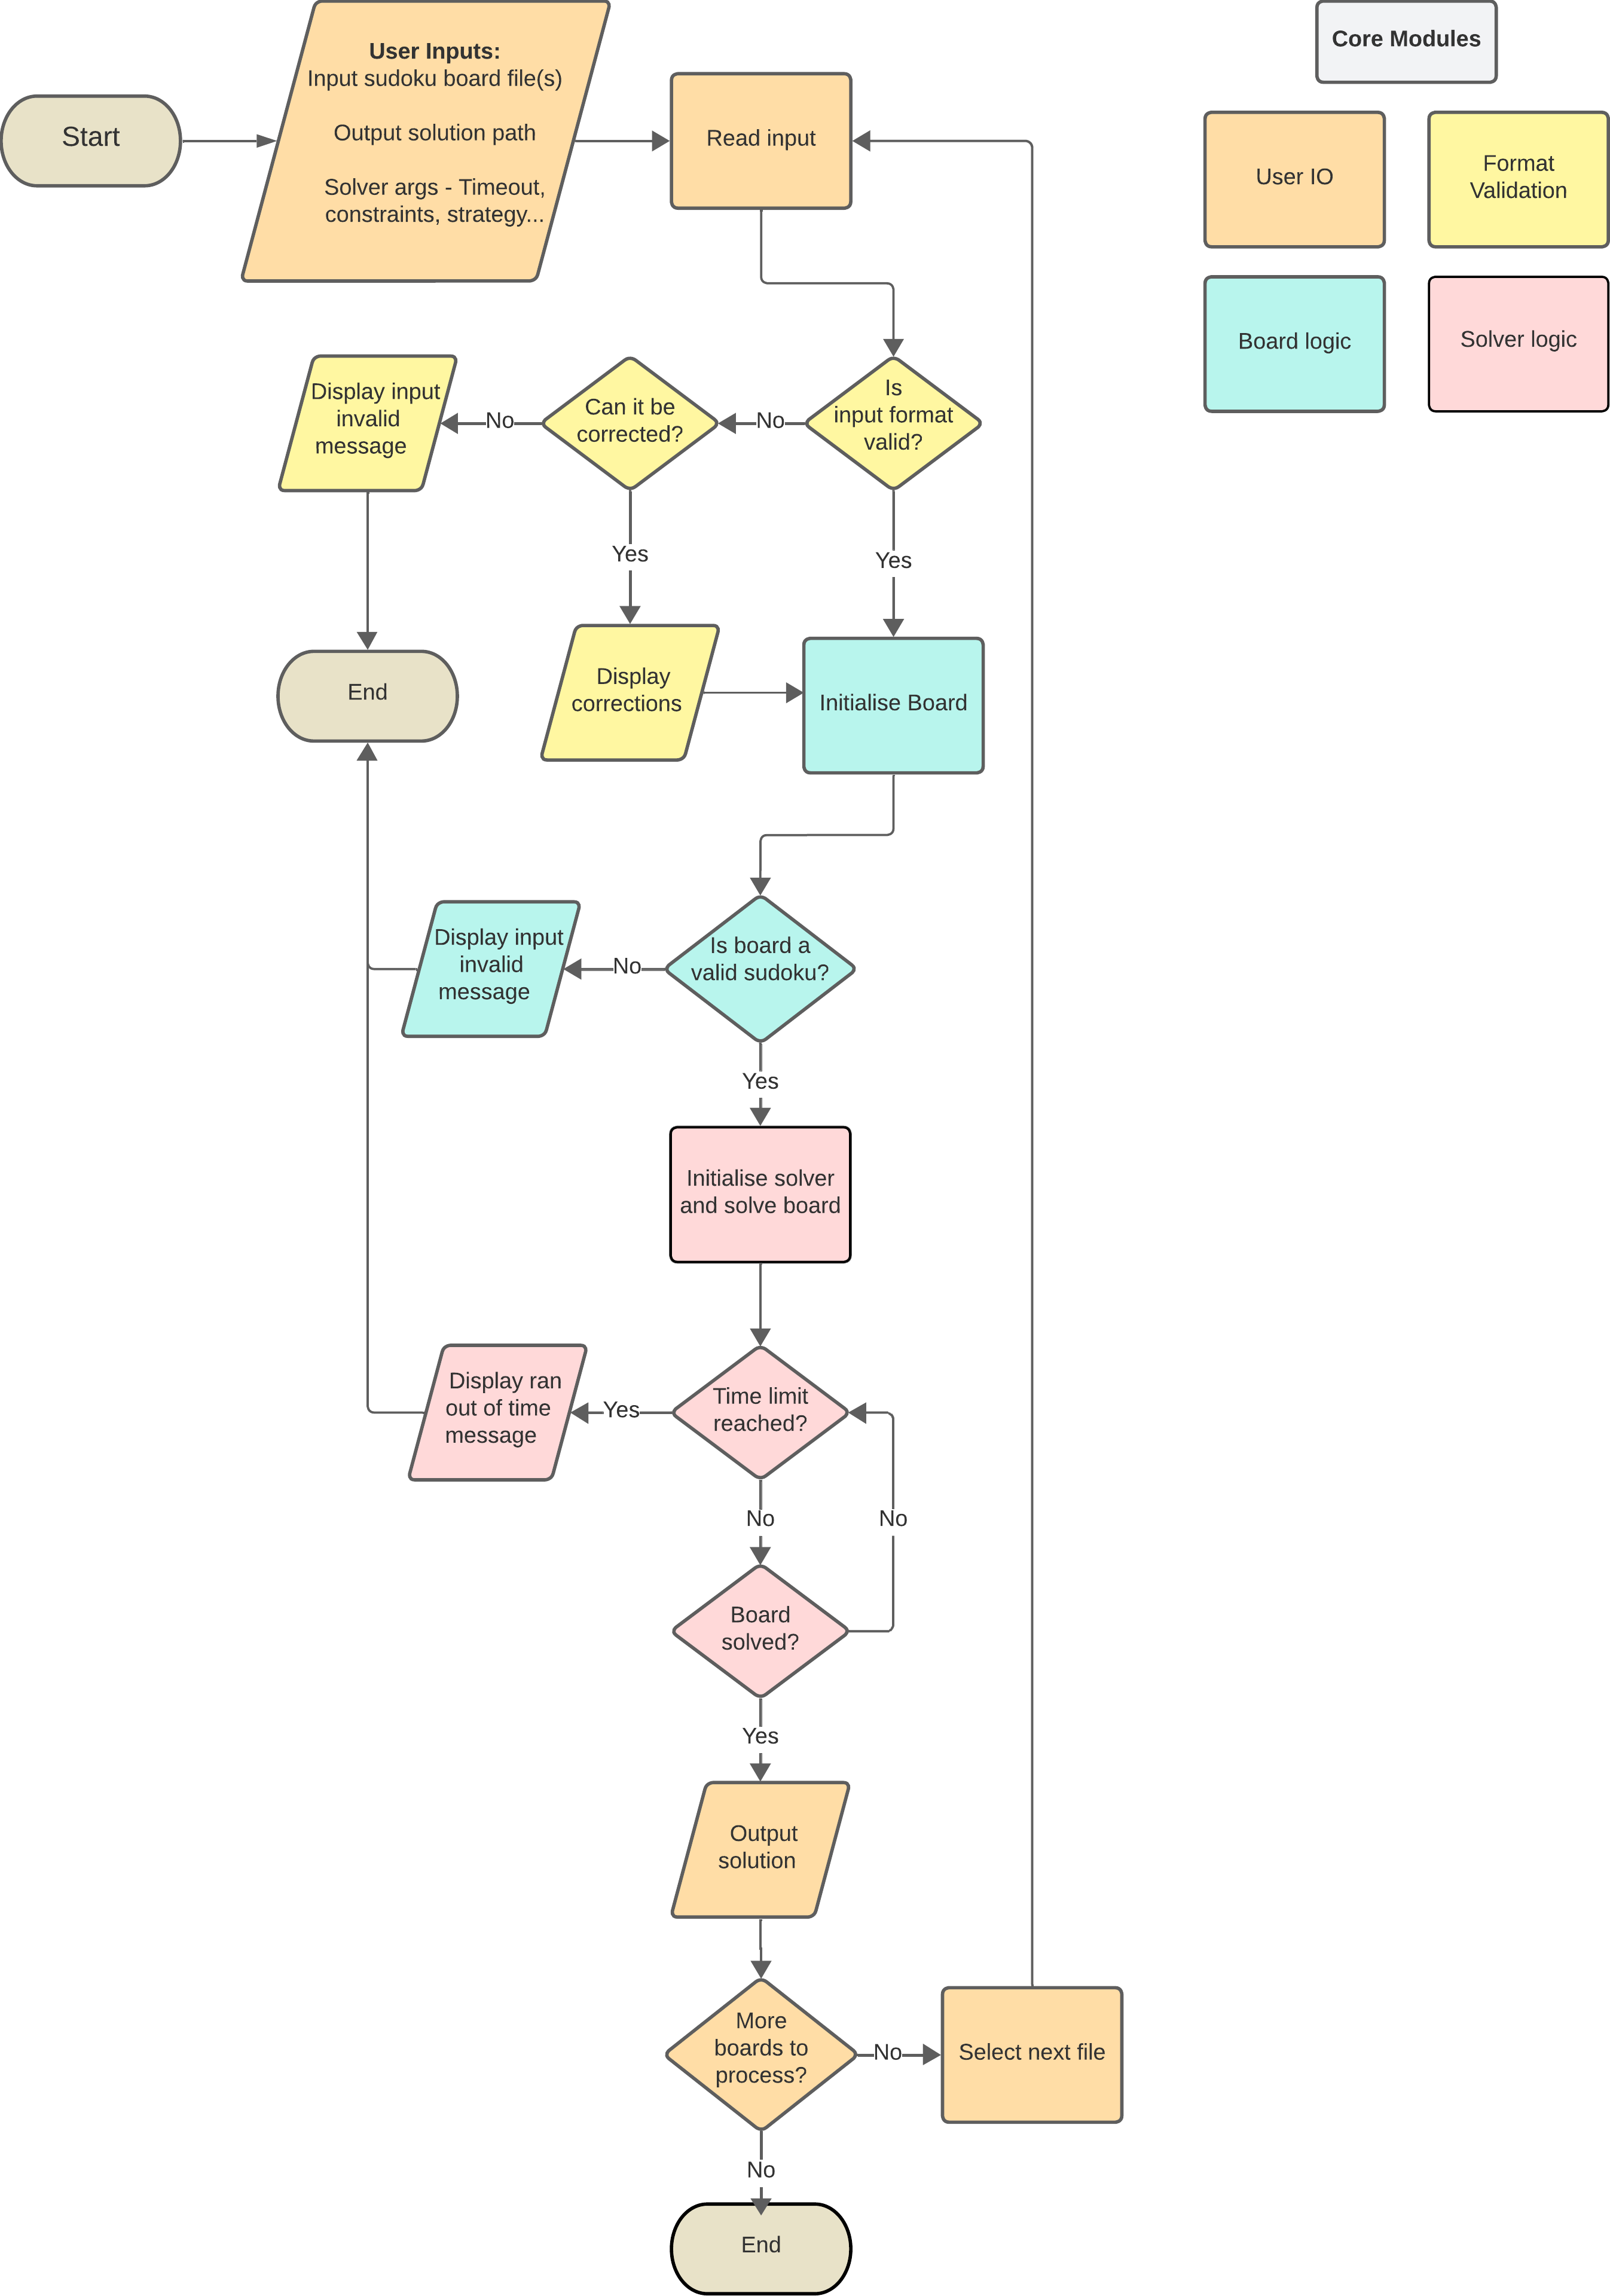
\includegraphics[width=1\textwidth]{figs/solver_flowchart.png}
\caption{High-level flowchart of the Sudoku solver program, illustrating the initial conceptual design. Functionally related modules are color-coded: orange for user interaction, yellow for format validation, cyan for board logic, and pink for solver logic components.}
\label{fig:solver_flowchart}
\end{figure}

The analysis led to the identification of the following key modular components in the Sudoku solver:

\begin{itemize}
\item \textbf{User IO:} Responsible for user interaction and input/output processing.
\item \textbf{Format Validation:} Ensures the correctness of the input format.
\item \textbf{Board Logic:} Manages the internal representation and manipulation of the Sudoku board.
\item \textbf{Solver Logic:} Implements the algorithms to solve the Sudoku puzzle.
\end{itemize}


\subsection{Developmental Journey}
Before delving into the final structure of the Sudoku solver, it is insightful to explore the initial prototyping phase. This phase laid the groundwork for the project and provided key insights that shaped the final design.

\subsubsection{Early Prototyping}
In the initial stages, the envisioned usage of the program was conceptualised as a straightforward sequence of operations involving board validation, board representation, and solving. The logical flow was as follows:

\begin{enumerate}
\item \textbf{Board Validation}: The user provides a file containing the Sudoku puzzle, which is then read, validated, and corrected if necessary. This process was handled by a utility function, \texttt{validate\_board}, located in the \texttt{utils} module. The function's purpose was to ensure the input adhered to Sudoku format standards and to correct any discrepancies. The code snippet for this step:
\begin{verbatim}
board_array = utils.validate_board(board_file)
\end{verbatim}
This function returns a 9x9 array representing the initial state of the Sudoku board.

\item \textbf{Board Representation}: The returned board array is then used to initialise an instance of the `\texttt{SudokuBoard}` class. This class encapsulates the board's representation and manipulation logic, providing common game board methods like `\texttt{reset}` and `\texttt{check\_valid}`. The initialisation step is shown below:
\begin{verbatim}
sudoku_board = SudokuBoard(board_array)
\end{verbatim}

\item \textbf{Solving the Puzzle}: Finally, the `\texttt{SudokuBoard}` instance is passed to the `\texttt{solve}` method of a `\texttt{BacktrackingSolver}` class instance. The solver applies the backtracking algorithm to find a solution to the puzzle, returning a new `\texttt{SudokuBoard}` instance representing the solved board:
\begin{verbatim}
solver = BacktrackingSolver().solve(board)
\end{verbatim}

\end{enumerate}

\subsubsection{Early Hurdles and Insights}
The initial testing of the program, particularly on diverse Sudoku puzzles, including a Kaggle dataset of a million boards, brought to light several key issues and limitations with the initial design. These challenges played a crucial role in shaping the subsequent development of the solver.

\paragraph{Modularity Challenges:}
One of the first hurdles encountered was the lack of modularity in handling board validation, correction, and parsing. The initial approach used a single utility function, `\texttt{validate\_board}`, which combined these processes. This lack of separation hindered flexibility and made it difficult to handle multiple input formats or to separate validation from parsing:

\paragraph{Supporting Multiple Input Formats:}
The project faced a significant challenge when dealing with input formats different from the expected grid-based format. Specifically, the Kaggle dataset was in a single line format, necessitating a conversion process to and from the grid format. This experience underscored the need for native support for multiple input formats and highlighted the inefficiency of the existing approach where saving and loading logic were tied to a specific format.

\paragraph{Evolution of SudokuBoard:}
The SudokuBoard class underwent significant refinement. Initially, it included some output logic, but it became clear that this class should focus solely on representing the Sudoku board and interfacing with solvers through methods like \texttt{get\_empty\_cells}, \texttt{check\_valid\_move}, and \texttt{reset\_board}. This realisation led to a cleaner and more focused class. It also took on some of the validation logic from the utility function that related to checking the input board followed the rules of Sudoku.

\paragraph{Solver Extensibility:}
Another insight gained was the need for a more flexible system to integrate new solver algorithms. The initial setup did not provide an easy way to select or initialise different solvers that may not share initialisation parameters, leading to potential difficulties in adding complex algorithms with unique initialisation requirements.

\paragraph{Enhancing Input Flexibility and User Options in main.py:}
The final insight was on making main.py more adaptable and user-friendly. The current script was designed for single file-based inputs however it needed to be able to accept both single puzzle file paths and directories containing multiple puzzles. Additionally, a desirable feature that was initially not thought to be signifcant was the incorporation of string input capability. This greatly facilitated quick puzzle testing from online sources. This feature allowed for direct copy-pasting of puzzles into the terminal, streamlining the validation process. Moreover, the script was adapted to enable dynamic selection and initialisation of various solvers and format handlers without the need for code modifications, thereby increasing the programs flexibility while maintaining modularity.
\subsubsection{High-Level Overview of the Final Implementation}
The final design of the Sudoku solver program encapsulates a modular and flexible architecture, as outlined below:

\begin{verbatim}
# Initialise the Format Handler and Solver
format_handler = SudokuFormatHandler()
solver = SudokuSolver()

# Parse the Sudoku board from the given input in the desired format
board = format_handler.parse(board_file, format_type)

# Employ a specific solver to find a solution for the parsed board 
solved_board = solver.solve(board, solver_backend)

# Save the solved board in the desired format and output path
format_handler.save(solved_board, format_type, output_path)
\end{verbatim}

In this design, \texttt{SudokuFormatHandler} and \texttt{SudokuSolver} act as wrapper classes that have methods which allow the user to specify which format and solver backend they want to use, respectively. These classes utilise standardised methods to process and solve the Sudoku puzzle, irrespective of the specific format or solving algorithm used. This approach significantly enhances the extensibility of the program, allowing for the easy integration of new formats and solving methods without requiring changes to the \texttt{main.py} script. Additionally, the flexibility to save the output in either the native format of the input or any other specified format is achieved by adjusting the \texttt{format\_type} argument, further increasing the program's versatility and user-friendliness. The next section will explore the design and implementation of the various modules in greater detail.

\section{Programme Modules}
\subsection{Class SudokuFormatHandler}

\subsubsection{Scope}
The scope of the FormatHandler classes implemented in \texttt{src/sudoku\_format\_handler.py} is defined by its role in bridging the gap between external representations of Sudoku boards and standardised internal representation. Specifically, the scope of this class encompasses:

\begin{itemize}
\item \textbf{Parsing}: Handling the conversion of the input, whether it comes as a string or as a file path, into a standardised \texttt{SudokuBoard} object.

\item \textbf{Saving}: Conversely, the class also manages the conversion of \texttt{SudokuBoard} objects back into user-readable formats. 

\item \textbf{Format Validation and Correction}: This class is also where the developer defines any methods for validation checks and corrections to ensure that the input is in the expected format before parsing.
\end{itemize}

\subsubsection{Design}
The design of the \texttt{SudokuFormatHandler} class is centered around principles of modularity and extensibility, driven by the use of an abstract base class and a handler dictionary. Key design aspects include:

\begin{itemize}
    \item \textbf{Modularity}: The class leverages an abstract base class, \texttt{FormatHandler}, which outlines essential methods -- \texttt{parse} and \texttt{save}. This structure ensures consistency across different format handlers while allowing for flexibility in their specific implementations.
    \item \textbf{Extensibility}: New formats can be easily integrated into the system by creating a subclass of \texttt{FormatHandler} and adding it to \texttt{SudokuFormatHandler}'s \texttt{handler\_dict} class attribute. This approach simplifies the process of extending the system to accommodate new Sudoku board formats.
    \item \textbf{Abstraction}: The abstract methods in \texttt{FormatHandler} enforce a contract that all subclasses must provide specific implementations for parsing and saving Sudoku boards, thus maintaining a standardised interface.
\end{itemize}
The UML class diagrams in Figure \ref{fig:format_handler_uml} provide a visual representation of the design and implementation of the \texttt{FormatHandler} abstract base class and the \texttt{SudokuFormatHandler} class, respectively.
\begin{figure}[H]
    \centering
    \includegraphics[width=1\textwidth]{figs/UML_sudoku_handler.png}
    \caption{Class diagram for the SudokuFormatHandler module, illustrating the design and implementation of the FormatHandler abstract base class and the SudokuFormatHandler class. Along with the composition of the SudokuFormatHandler class with the implemented Format classes (GridFormatHandler and FlatFormatHandler).}
    \label{fig:format_handler_uml}
\end{figure}

\subsubsection{Implementation}
The implementation of \texttt{SudokuFormatHandler} involves several key components that collectively enable dynamic handling of various board formats:

\begin{itemize}
    \item \textbf{Handler Dictionary}: The \texttt{handler\_dict} serves as a central repository linking format types (e.g., 'grid', 'flat') to their corresponding handler objects, facilitating the flexible handling of different formats.
    \item \textbf{Handler Retrieval}: The method \texttt{\_get\_handler} takes a format type as input and retrieves the appropriate handler from \texttt{handler\_dict}. It raises a \texttt{KeyError} with available format options in case of an unsupported format type.
    \item \textbf{Parse Method}: The \texttt{parse} method interfaces with the selected handler to transform the input into a \texttt{SudokuBoard} object. It delegates the specifics of parsing to the corresponding format handler.
    \item \textbf{Save Method}: Similarly, the \texttt{save} method utilizes the appropriate handler to convert a \texttt{SudokuBoard} object back into a file, ensuring consistency in the output process across different input formats.
\end{itemize}


\subsubsection{Extensibility}
The\texttt{SudokuFormatHandler} is designed with extensibility in mind. To support a new format, a developer simply needs to create a new handler class extending \texttt{FormatHandler} and implement the \texttt{parse} and \texttt{save} methods with the expected inputs and outputs. The new handler can then be added to the \texttt{handler\_dict}. This design makes it straightforward to extend the solver's capabilities to accommodate future requirements or user preferences for different Sudoku board formats.


\subsubsection{Limitations}
The current design of the SudokuFormatHandler module, as well as other related modules, is specifically tailored to process single Sudoku boards from individual input files. This intentional design choice is due to the significant increase in complexity that would arise from trying to build a general framework which supports multiple formats that also supports accommodating multiple boards within a single file. Maintaining a single input, single board paradigm simplifies the overall program structure and aligns with our current functional objectives. 


\subsection{SudokuBoard Class}
Future work is to make a board abc for future representations like dictionary based boards

\subsubsection{Scope of the SudokuBoard Class}
The \texttt{SudokuBoard} class in \texttt{src/sudoku\_board.py} is integral to managing the internal representation and manipulation of the Sudoku board and providing a standardised interface for the other classes in the program. The scope of this class encompasses:

\begin{itemize}
    \item \textbf{Board Validation}: Makes sure board state always follows Sudoku rules. 
    \item \textbf{Board Representation}: Provides a standardised representation of the board state for the other classes. 
    \item \textbf{Board Manipulation}: Facilitates methods for resetting the board and modifying cell values to allow for board manipulation.
    \item \textbf{Solving Assistance}: Provides common utility methods required by typical solvers, such as fetching empty cells and checking valid number placements.

\end{itemize}
\subsubsection{Design}
The design of the \texttt{SudokuBoard} class is centered around the principle of encapsulation. The other classes in the program interact with the board through a standardised interface of class methods, without needing to know the internal representation or logic. Key design aspects include:


\subsection{SudokuSolver Class}

\subsection{main.py}

\section {Testing and Optimisation}
\subsection {Profiling}

\section {SWE}
Unit Tests and CI set up
Packaging and Usability

\section {Summary}

% \subsection{Scope}
% The User IO module serves as the primary interface between the user and the Sudoku solver program. Its responsibilities include:

% \begin{itemize}
% \item Collecting user input.
% \item Validating user input.
% \item Displaying the output of the program.
% \item Saving the output of the program.
% \end{itemize}

% \subsection{Design Considerations}
% Contrary to the development order, the User IO module's design was influenced significantly by prior interaction with other modules. This sequential approach ensured a more user-centric design, accommodating the needs identified through initial module interactions.

% \subsubsection{User Input Flexibility}
% A key feature of this module is its flexibility in accepting user input, either directly as a string or via a filepath. This was driven by the practical need to quickly test Sudoku boards obtained from various sources, often online. Additionally, the design allows for effortless expansion to accommodate new solvers or input formats.

% \subsection{Operational Modes}
% The User IO module supports two primary modes of operation:

% \begin{itemize}
% \item \textbf{Single Input Mode}: For individual puzzle solving, this mode is optimised for ease of use, requiring minimal parameters.
% \item \textbf{Batch Testing Mode}: Geared towards performance analysis, this mode facilitates processing multiple puzzles from a directory, with options for output saving and detailed statistical analysis.
% \end{itemize}

% \subsection{Future Extensibility and Reproducibility}
% The current implementation of solvers is straightforward, with a single timeout parameter. However, the design anticipates more complex solvers in the future. A specific section in main.py is earmarked for integrating such enhancements, potentially through a configuration file mechanism.

% To aid in the reproducibility of runs, particularly for performance comparison across different solver versions, the module captures and stores the git commit hash and run arguments in the output summaries.

% \subsection{Implementation Strategy}
% The module is implemented as a set of functions in the main.py script, favoring function-based design over a class-based approach. This decision was driven by the need for rapid prototyping and ease of adding new features.

% A high level overview of the implementation is shown in figure
% \subsubsection{Argument Parsing}
% Using argparse, the script effectively handles various user inputs. The design ensures that the most straightforward use case—solving a single puzzle—requires the least user input. Additional options like output path and run statistics are available for deeper analysis. The batch mode is specifically tailored for performance testing, generating comprehensive statistical data for each puzzle in the dataset.


% \subsubsection{Backend Integration}
% As the backend evolves with new solvers and input formats, these enhancements are automatically integrated into the User IO module, demonstrating the system's extensible and user-centric architecture.
% Uncomment the following two lines if you have references
%\bibliographystyle{plain}
%\bibliography{references}

\end{document}
